\section{Models}
With the question defined, the equations of motion derived, we can now consider the different models to achieve maximum displacement from a single jump.

% TODO: maybe put the constants before engine section
\subsection{Constants}
One might notice that I've deliberately left some of the constants $j_i$ clear of meaningful values and only suggested in-game default values. This is because many long-jumpers in the community find the default (vanilla) settings of the game engines ``bland'', reducing the excitement of this activity. Therefore, I will be setting some of the engine constants myself.

There are 4 of them:
\begin{itemize}
    \item \verb|sv_gravity| ($g$), set to 800
    \item \verb|sv_maxspeed| ($L$), set to 250
    \item \verb|sv_airaccelerate| ($A$), set to 12
    \item \verb|tickrate| ($n$), set to 64, or $\tau=\frac{1}{64}$
\end{itemize}

The only meaning deviation from the default settings are the speed limit $L$, for the default settings limits the optimization one can achieve, while the higher value of $250$ simply magnifies the result that one can achieve.

Furthermore, all models are free to set the initial velocity $\tv_0$, with the constraint that the magnitude of $\tv_0$ does not exceed $250$, the speed limit.

\subsection{Straight line}
% where you do nothing
We all know the fastest route (shortest distance) from point $A$ to point $B$ is with a straight line connecting $A$ to $B$. Therefore if the velocity magnitude is maximized, and as time is proportional to distance: $t = \frac{s}{\tmag{\tv}}$, it seems that a straight line would maximize the jumping distance assuming no constraints. This will serve as a good baseline for all the other models.

I have decided for the player to travel along the y-axis because I personally find it nicer to graph and draw with, but all maths would apply if you wish to substitute for the x-axis. This is represented by the acceleration function:

\begin{figure}[H]
    \centering
    \[
    \tunit{a}(t) = \tang{0, 1}
    \]
    \caption{The straight line model}
\end{figure}

Notice that player acceleration is constant in this model, and which can be achieved simply by looking forward, and press the key $w$ during the jump. Furthermore, we can set the initial velocity to point directly upwards in the y direction, such that:
\[
\tv_0 = \tang{0, 250},
\]
for common knowledge tells me that a faster initial speed in the direction where I am going will result in higher overall travel distance. Overall, there exists four metrics for each model, each worth evaluating.

We can first look at the case without the max speed constraint. By running a simulation with the engine constants discussed before, I got a result of $\approx 933.84$ hammer units in a jump. Predictably, this model will have the player traveling in a straight line (figure \ref{fig:straight_nothing_1}).

\begin{wrapfigure}{r}{0.5\textwidth}
    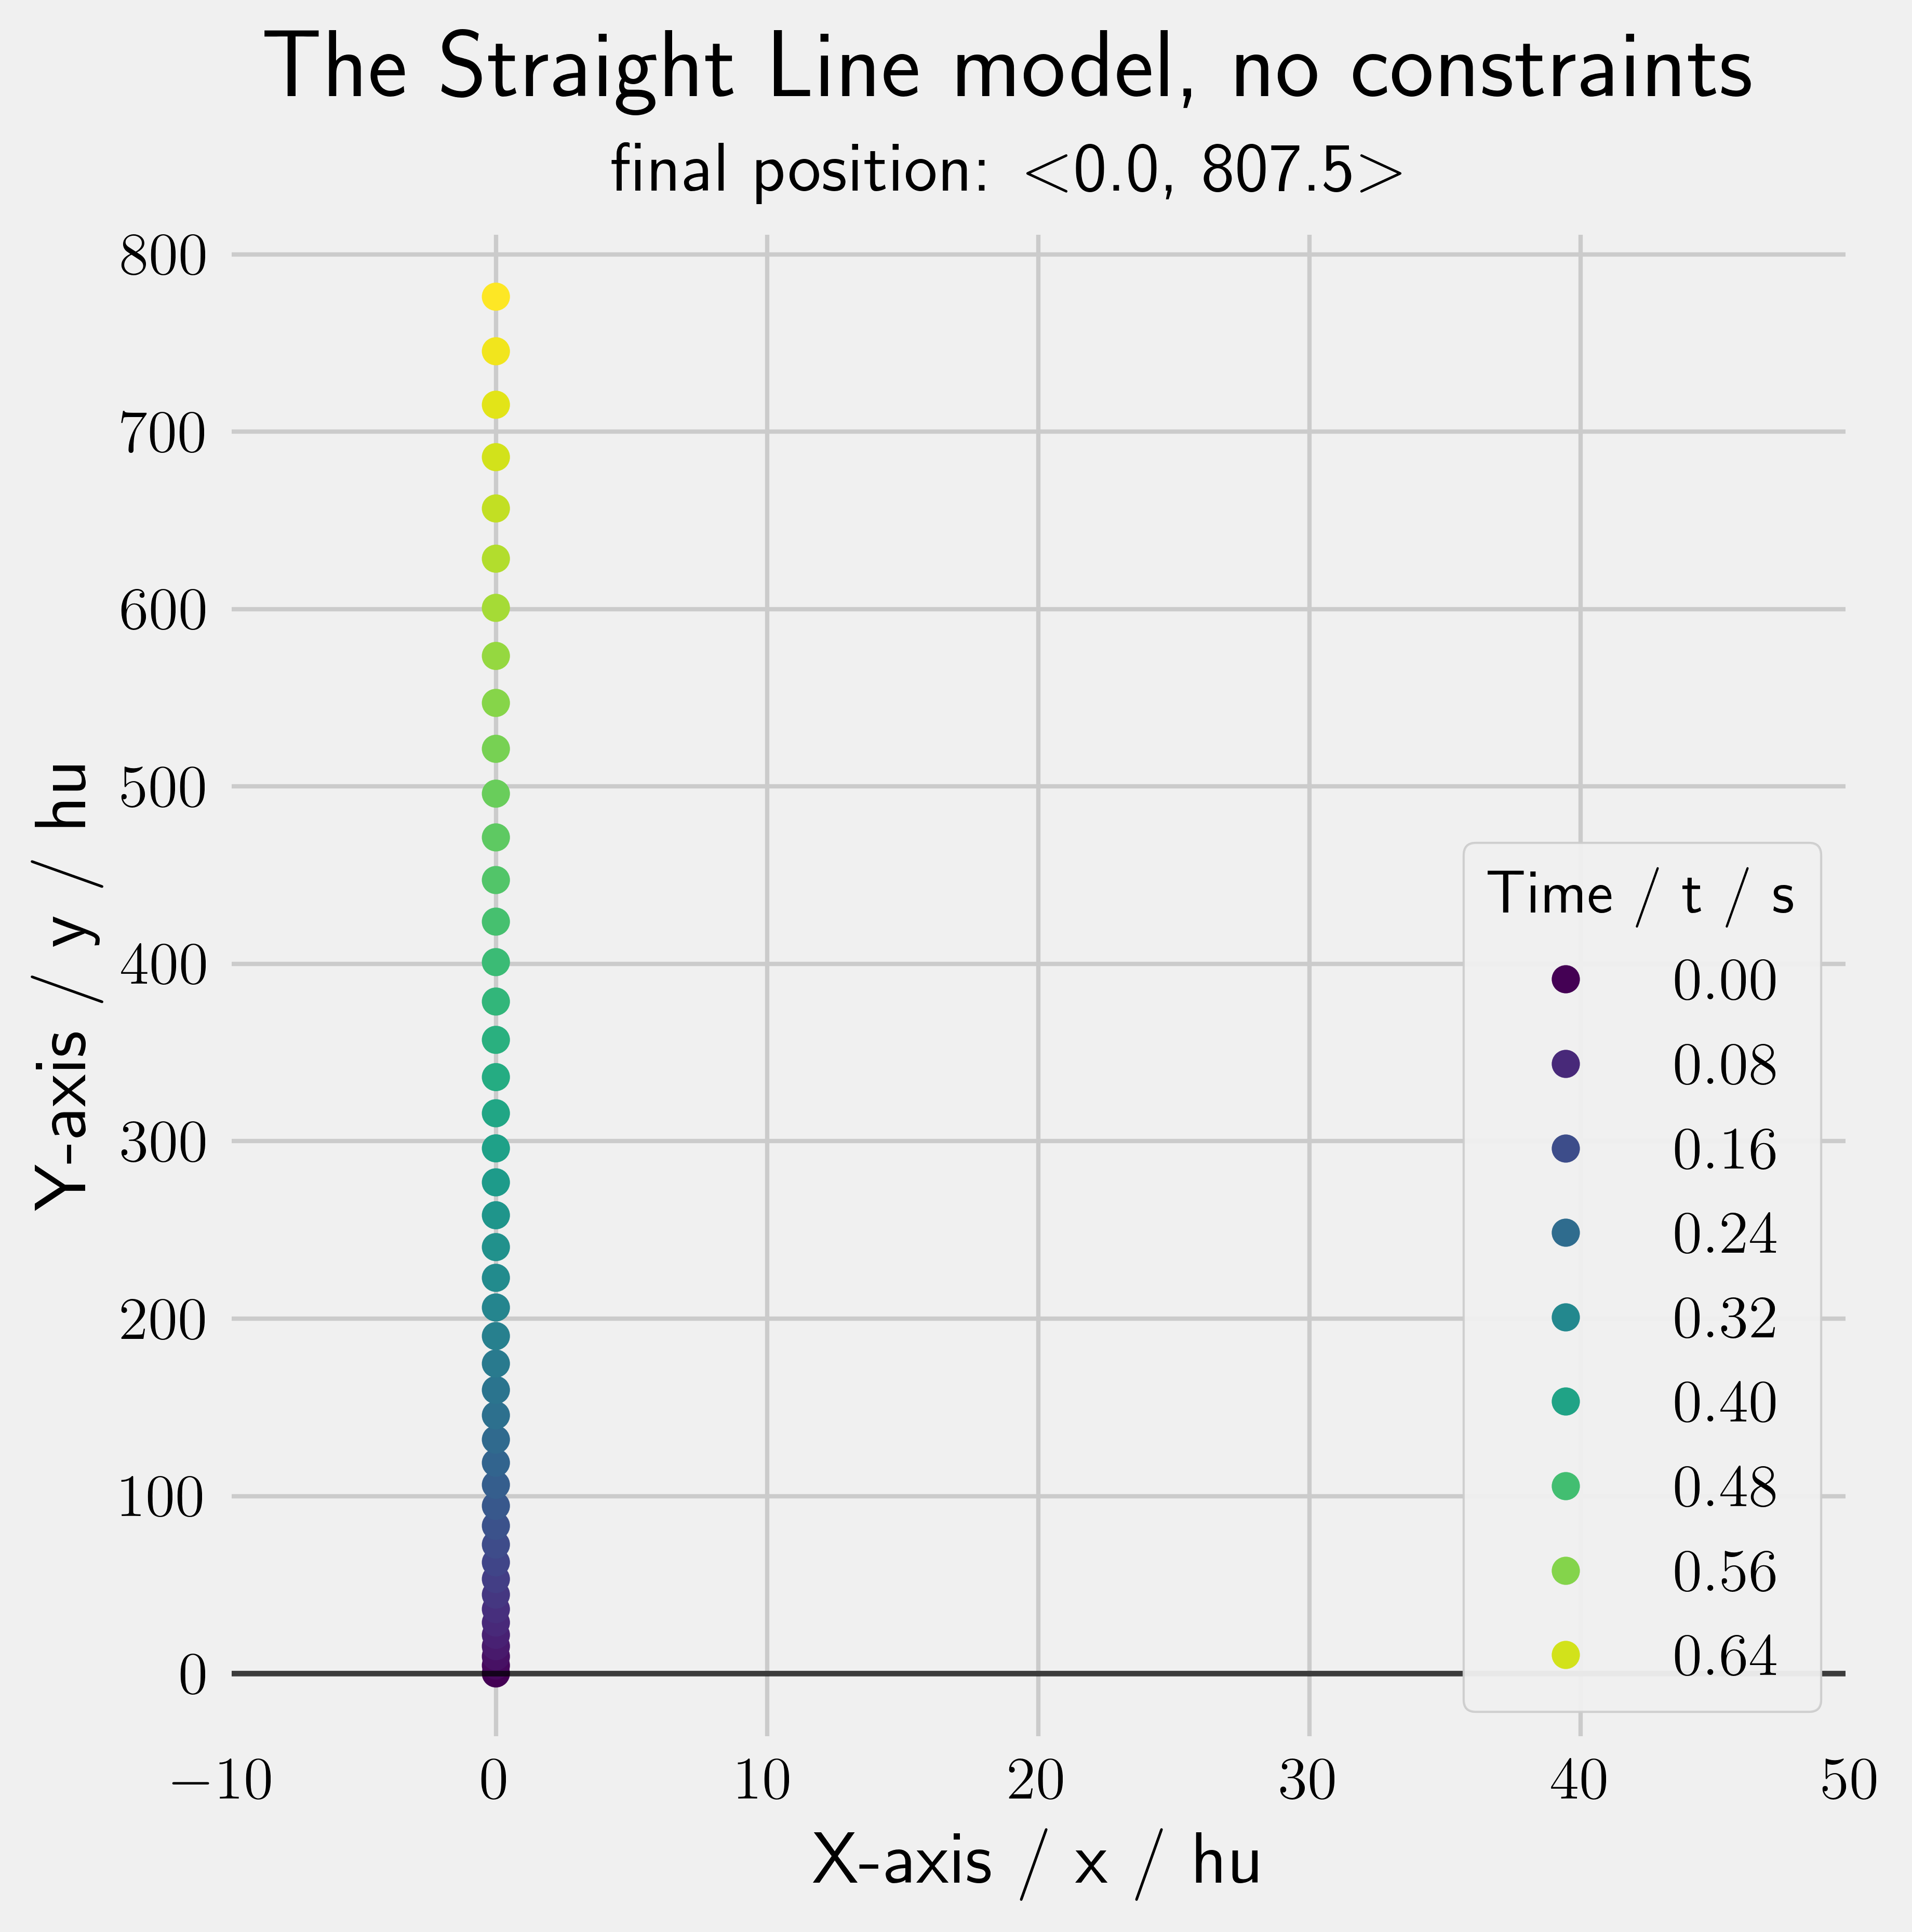
\includegraphics[width=0.48\textwidth,right]{assets/straight_nothing_1.png}
    \caption{}
    \label{fig:straight_nothing_1}
\end{wrapfigure}

I can comfortably say that this jumping distance would never be possible to achieve in game, for this model can be proven to be the most optimal jumping path if there are no speed limits (appendix, using EL equation). This number of around $900$ hammer units serves to be the upper-bound of our optimization, and the lower-bound being its inverse of
